\documentclass{ime-beamer}
\usepackage[portuges]{babel}
\usepackage[utf8]{inputenc}
\usepackage{graphicx}
\usepackage[portuguese]{algorithm2e}% Para escrever algorítimos
\usepackage{listings}			% Para usar \lstinputlisting e incluir código
\usepackage{subcaption}			% Para usar \begin{subfigure} e colocar figuras (a) e (b) lado a lado
\usepackage{multicol}

\title[Técnicas de IA aplicadas ao futebol de robôs]{%
  Técnicas de IA Aplicadas a Sistemas Multiagentes Cooperativos e Competitivos
}
\author[Jan Segre\and Victor Bramigk]{%
  Jan Segre\\
  Victor Bramigk\\
  Paulo F. F. Rosa (Orientador)\\
  Bruno Madeira (Co-orientador)
}

% as imagens ficam nesse diretório
\graphicspath{{img/}}

\begin{document}
\frame{\maketitle}

\frame{%
  \frametitle{Roteiro}
  \tableofcontents
}

\section{Introdução}
% tempo: 1 min
% Robocup / Roboime /ssl
% Objetivo
% Estudo do Minimax
% Modelagem ( contínuo -> discreto )
% Prova de Conceito
\frame{%
  \frametitle{Robocup}
  \begin{block}{}
    \begin{figure}
      \centering
      \includegraphics[width=0.7\linewidth]{robocup2013}
      \caption{Imagem da SSL \textit{RoboCup} 2013 em Eindhoven, na Holanda}\label{fig:robocup2013}
    \end{figure}
  \end{block}
}

\section{Mapeamento para um jogo discreto}
% Modelagem
% tempo: 3 min
% - Nesce para entender o programa
% - Actions -> Tactics (Skills?)
% - Posse de bola
% - Move Pass Kick
\frame{%
  \frametitle{Mapeamento para um jogo discreto}
  \begin{block}{}
    \centering
    Mapear um jogo contínuo em tempo e espaço para um jogo discreto em pelo
    menos no tempo, isto é, jogadas bem definidas.
  \end{block}
}
\frame{%
  \frametitle{Mapeamento para um jogo discreto}
  \begin{block}{}
    \centering
    Mapeamento proposto:

    \begin{itemize}
      \item Ação de um time com a bola é uma lista de:
        \begin{itemize}
          \item robô sem a bola:
            \begin{itemize}
              \item $Move(x, y)$
            \end{itemize}
          \item robô com a bola:
            \begin{itemize}
              \item $Kick(x, y)$
              \item $Pass(r)$
            \end{itemize}
        \end{itemize}
      \item Ação de um time sem a bola é uma lista de:
        \begin{itemize}
          \item $Move(x, y)$
        \end{itemize}
    \end{itemize}
  \end{block}
}

\section{Arquitetura}
% tempo: 4 min
% - Armadillo
% - compet. ???
% - zmq / rede
% - evidenciar vantagens
% - python / c++
% - concluir que faz mais sentido
\frame{%
  \frametitle{Arquitetura}
  \begin{block}{}
    \begin{figure}
      \centering
      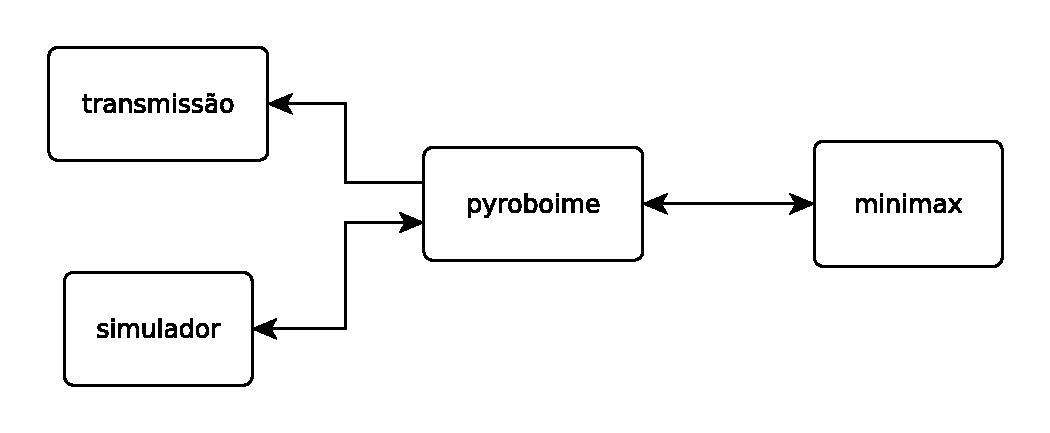
\includegraphics[width=0.8 \linewidth]{img/arq_geral_prog}
      \caption{Arquitetura simplificada do sistema de controle}\label{fig:arq_prog}
    \end{figure}
  \end{block}
}

\section{Programa}
% Modelagem
% tempo: 5 min
% - exemplo representacao
% - funcao de avaliacao e dados auxiliares
% - exemplo passe
% - execucao no grsim
\frame{%
  \frametitle{Programa}
  \begin{block}{}
  \end{block}
}


\setlength{\tabcolsep}{3pt}
\section{Cronograma}
\frame{%
  \frametitle{Cronograma}
  \begin{table}[Ht!]
    \begin{center}
      \begin{tabular}{|*{12}{c|}}
      \hline &    \multicolumn{5}{|c|}{2014}   &             \multicolumn{6}{|c|}{2015}           \\ \hline
      Tarefas& Ago   & Set   & Out    & Nov    & Dez   & Jan   & Fev  & Mar  & Abr  & Mai  & Jun  \\ \hline
      \hline
      MMP    &   X   &   X   &   X    &        &       &       &      &      &      &      &      \\ \hline
      PVC    &       &       &   X    &   X    &       &       &      &      &      &      &      \\ \hline
      IMPARQ &       &       &   X    &   X    &   .   &       &      &      &      &      &      \\ \hline
      IMPALG &       &       &        &        &   .   &   .   &   .  &   .  &   .  &      &      \\ \hline
      TST    &       &       &        &        &       &       &   .  &   .  &   .  &      &  PR  \\ \hline
      RED    &   X   &   X   &   X    &   X    &   .   &   .   &   .  &   .  &   .  &      &      \\ \hline
      DEF    &       &       &        &        &       &       &      &      &      &   .  &      \\ \hline
    \end{tabular}
    \end{center}
  \end{table}
}

\section{Conclusão}
\frame{%
  \frametitle{Conclusão}
  \begin{block}{}
  \end{block}
}
\end{document}
% vim: tw=80 et ts=2 sw=2 sts=2
